\documentclass[twoside]{book}

% Packages required by doxygen
\usepackage{fixltx2e}
\usepackage{calc}
\usepackage{doxygen}
\usepackage[export]{adjustbox} % also loads graphicx
\usepackage{graphicx}
\usepackage[utf8]{inputenc}
\usepackage{makeidx}
\usepackage{multicol}
\usepackage{multirow}
\PassOptionsToPackage{warn}{textcomp}
\usepackage{textcomp}
\usepackage[nointegrals]{wasysym}
\usepackage[table]{xcolor}

% Font selection
\usepackage[T1]{fontenc}
\usepackage[scaled=.90]{helvet}
\usepackage{courier}
\usepackage{amssymb}
\usepackage{sectsty}
\renewcommand{\familydefault}{\sfdefault}
\allsectionsfont{%
  \fontseries{bc}\selectfont%
  \color{darkgray}%
}
\renewcommand{\DoxyLabelFont}{%
  \fontseries{bc}\selectfont%
  \color{darkgray}%
}
\newcommand{\+}{\discretionary{\mbox{\scriptsize$\hookleftarrow$}}{}{}}

% Page & text layout
\usepackage{geometry}
\geometry{%
  a4paper,%
  top=2.5cm,%
  bottom=2.5cm,%
  left=2.5cm,%
  right=2.5cm%
}
\tolerance=750
\hfuzz=15pt
\hbadness=750
\setlength{\emergencystretch}{15pt}
\setlength{\parindent}{0cm}
\setlength{\parskip}{3ex plus 2ex minus 2ex}
\makeatletter
\renewcommand{\paragraph}{%
  \@startsection{paragraph}{4}{0ex}{-1.0ex}{1.0ex}{%
    \normalfont\normalsize\bfseries\SS@parafont%
  }%
}
\renewcommand{\subparagraph}{%
  \@startsection{subparagraph}{5}{0ex}{-1.0ex}{1.0ex}{%
    \normalfont\normalsize\bfseries\SS@subparafont%
  }%
}
\makeatother

% Headers & footers
\usepackage{fancyhdr}
\pagestyle{fancyplain}
\fancyhead[LE]{\fancyplain{}{\bfseries\thepage}}
\fancyhead[CE]{\fancyplain{}{}}
\fancyhead[RE]{\fancyplain{}{\bfseries\leftmark}}
\fancyhead[LO]{\fancyplain{}{\bfseries\rightmark}}
\fancyhead[CO]{\fancyplain{}{}}
\fancyhead[RO]{\fancyplain{}{\bfseries\thepage}}
\fancyfoot[LE]{\fancyplain{}{}}
\fancyfoot[CE]{\fancyplain{}{}}
\fancyfoot[RE]{\fancyplain{}{\bfseries\scriptsize Generated by Doxygen }}
\fancyfoot[LO]{\fancyplain{}{\bfseries\scriptsize Generated by Doxygen }}
\fancyfoot[CO]{\fancyplain{}{}}
\fancyfoot[RO]{\fancyplain{}{}}
\renewcommand{\footrulewidth}{0.4pt}
\renewcommand{\chaptermark}[1]{%
  \markboth{#1}{}%
}
\renewcommand{\sectionmark}[1]{%
  \markright{\thesection\ #1}%
}

% Indices & bibliography
\usepackage{natbib}
\usepackage[titles]{tocloft}
\setcounter{tocdepth}{3}
\setcounter{secnumdepth}{5}
\makeindex

% Hyperlinks (required, but should be loaded last)
\usepackage{ifpdf}
\ifpdf
  \usepackage[pdftex,pagebackref=true]{hyperref}
\else
  \usepackage[ps2pdf,pagebackref=true]{hyperref}
\fi
\hypersetup{%
  colorlinks=true,%
  linkcolor=blue,%
  citecolor=blue,%
  unicode%
}

% Custom commands
\newcommand{\clearemptydoublepage}{%
  \newpage{\pagestyle{empty}\cleardoublepage}%
}

\usepackage{caption}
\captionsetup{labelsep=space,justification=centering,font={bf},singlelinecheck=off,skip=4pt,position=top}

%===== C O N T E N T S =====

\begin{document}

% Titlepage & ToC
\hypersetup{pageanchor=false,
             bookmarksnumbered=true,
             pdfencoding=unicode
            }
\pagenumbering{alph}
\begin{titlepage}
\vspace*{7cm}
\begin{center}%
{\Large Zia A\+PI }\\
\vspace*{1cm}
{\large Generated by Doxygen 1.8.13}\\
\end{center}
\end{titlepage}
\clearemptydoublepage
\pagenumbering{roman}
\tableofcontents
\clearemptydoublepage
\pagenumbering{arabic}
\hypersetup{pageanchor=true}

%--- Begin generated contents ---
\chapter{Namespace Index}
\section{Namespace List}
Here is a list of all documented namespaces with brief descriptions\+:\begin{DoxyCompactList}
\item\contentsline{section}{\hyperlink{namespacezany}{zany} }{\pageref{namespacezany}}{}
\end{DoxyCompactList}

\chapter{Hierarchical Index}
\section{Class Hierarchy}
This inheritance list is sorted roughly, but not completely, alphabetically\+:\begin{DoxyCompactList}
\item \contentsline{section}{zany\+:\+:Pipeline\+:\+:Hooks}{\pageref{classzany_1_1_pipeline_1_1_hooks}}{}
\item \contentsline{section}{zany\+:\+:Pipeline\+:\+:Instance}{\pageref{classzany_1_1_pipeline_1_1_instance}}{}
\item \contentsline{section}{zany\+:\+:Interface\+Context}{\pageref{classzany_1_1_interface_context}}{}
\begin{DoxyCompactList}
\item \contentsline{section}{zany\+:\+:Context}{\pageref{classzany_1_1_context}}{}
\end{DoxyCompactList}
\item \contentsline{section}{zany\+:\+:Pipeline}{\pageref{classzany_1_1_pipeline}}{}
\item \contentsline{section}{zany\+:\+:Pipeline\+:\+:Set}{\pageref{classzany_1_1_pipeline_1_1_set}}{}
\end{DoxyCompactList}

\chapter{Class Index}
\section{Class List}
Here are the classes, structs, unions and interfaces with brief descriptions\+:\begin{DoxyCompactList}
\item\contentsline{section}{\hyperlink{classzany_1_1_context}{zany\+::\+Context} \\*One implementation of context }{\pageref{classzany_1_1_context}}{}
\item\contentsline{section}{\hyperlink{classzany_1_1_pipeline_1_1_hooks}{zany\+::\+Pipeline\+::\+Hooks} }{\pageref{classzany_1_1_pipeline_1_1_hooks}}{}
\item\contentsline{section}{\hyperlink{classzany_1_1_pipeline_1_1_instance}{zany\+::\+Pipeline\+::\+Instance} }{\pageref{classzany_1_1_pipeline_1_1_instance}}{}
\item\contentsline{section}{\hyperlink{classzany_1_1_interface_context}{zany\+::\+Interface\+Context} }{\pageref{classzany_1_1_interface_context}}{}
\item\contentsline{section}{\hyperlink{classzany_1_1_pipeline}{zany\+::\+Pipeline} }{\pageref{classzany_1_1_pipeline}}{}
\item\contentsline{section}{\hyperlink{classzany_1_1_pipeline_1_1_set}{zany\+::\+Pipeline\+::\+Set} }{\pageref{classzany_1_1_pipeline_1_1_set}}{}
\end{DoxyCompactList}

\chapter{File Index}
\section{File List}
Here is a list of all documented files with brief descriptions\+:\begin{DoxyCompactList}
\item\contentsline{section}{lib/{\bfseries Zany.\+hpp} }{\pageref{_zany_8hpp}}{}
\item\contentsline{section}{lib/\+Zany/\hyperlink{_context_8hpp}{Context.\+hpp} \\*Execution queue of the tasks }{\pageref{_context_8hpp}}{}
\item\contentsline{section}{lib/\+Zany/{\bfseries Entity.\+hpp} }{\pageref{_entity_8hpp}}{}
\item\contentsline{section}{lib/\+Zany/{\bfseries Event.\+hpp} }{\pageref{_event_8hpp}}{}
\item\contentsline{section}{lib/\+Zany/{\bfseries Http\+Base.\+hpp} }{\pageref{_http_base_8hpp}}{}
\item\contentsline{section}{lib/\+Zany/{\bfseries Http\+Header.\+hpp} }{\pageref{_http_header_8hpp}}{}
\item\contentsline{section}{lib/\+Zany/{\bfseries Loader.\+hpp} }{\pageref{_loader_8hpp}}{}
\item\contentsline{section}{lib/\+Zany/{\bfseries Orchestrator.\+hpp} }{\pageref{_orchestrator_8hpp}}{}
\item\contentsline{section}{lib/\+Zany/\hyperlink{_pipeline_8hpp}{Pipeline.\+hpp} \\*Execution queue of the tasks }{\pageref{_pipeline_8hpp}}{}
\item\contentsline{section}{lib/\+Zany/{\bfseries Platform.\+hpp} }{\pageref{_platform_8hpp}}{}
\item\contentsline{section}{lib/\+Zany/{\bfseries Property.\+hpp} }{\pageref{_property_8hpp}}{}
\item\contentsline{section}{lib/\+Zany/{\bfseries Thread\+Pool.\+hpp} }{\pageref{_thread_pool_8hpp}}{}
\item\contentsline{section}{lib/\+Zany/\+Event/{\bfseries Event.\+hpp} }{\pageref{_event_2_event_8hpp}}{}
\item\contentsline{section}{lib/\+Zany/\+Event/{\bfseries Hdl\+Collector.\+hpp} }{\pageref{_hdl_collector_8hpp}}{}
\item\contentsline{section}{lib/\+Zany/\+Event/{\bfseries Manager.\+hpp} }{\pageref{_manager_8hpp}}{}
\end{DoxyCompactList}

\chapter{Namespace Documentation}
\hypertarget{namespacezany}{}\section{zany Namespace Reference}
\label{namespacezany}\index{zany@{zany}}
\subsection*{Classes}
\begin{DoxyCompactItemize}
\item 
class \hyperlink{classzany_1_1_context}{Context}
\begin{DoxyCompactList}\small\item\em One implementation of context. \end{DoxyCompactList}\item 
class \hyperlink{classzany_1_1_interface_context}{Interface\+Context}
\item 
class \hyperlink{classzany_1_1_pipeline}{Pipeline}
\end{DoxyCompactItemize}


\subsection{Detailed Description}
Namespace of the project 
\chapter{Class Documentation}
\hypertarget{classzany_1_1_context}{}\section{zany\+:\+:Context Class Reference}
\label{classzany_1_1_context}\index{zany\+::\+Context@{zany\+::\+Context}}


One implementation of context.  




{\ttfamily \#include $<$Context.\+hpp$>$}



Inheritance diagram for zany\+:\+:Context\+:\nopagebreak
\begin{figure}[H]
\begin{center}
\leavevmode
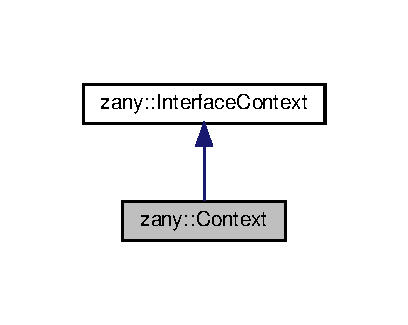
\includegraphics[width=196pt]{classzany_1_1_context__inherit__graph}
\end{center}
\end{figure}


Collaboration diagram for zany\+:\+:Context\+:\nopagebreak
\begin{figure}[H]
\begin{center}
\leavevmode
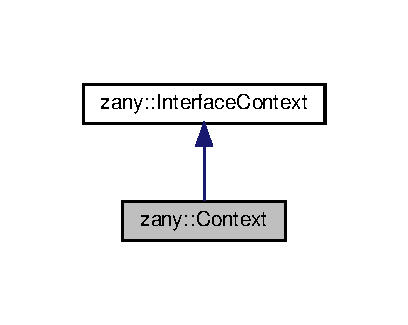
\includegraphics[width=196pt]{classzany_1_1_context__coll__graph}
\end{center}
\end{figure}
\subsection*{Public Member Functions}
\begin{DoxyCompactItemize}
\item 
\hyperlink{classzany_1_1_context_aed673136ee170788d0cd5717857c81c4}{Context} ()=default
\item 
\hyperlink{classzany_1_1_context_aaf02dd357e71f0608f6c034c5222930c}{Context} (\hyperlink{classzany_1_1_context}{Context} const \&other)=delete
\item 
\hyperlink{classzany_1_1_context_a0f3ea7fa76d75e239ac8ec95a517822e}{Context} (\hyperlink{classzany_1_1_context}{Context} \&\&other)=default
\item 
\hyperlink{classzany_1_1_context}{Context} \& \hyperlink{classzany_1_1_context_a35af38bc82dcac073aa0dbc0acca032d}{operator=} (\hyperlink{classzany_1_1_context}{Context} const \&other)=delete
\item 
virtual void \hyperlink{classzany_1_1_context_a448dcb8a627491eb4c8de0f46cd13ab1}{add\+Task} (Handler const \&handler) final
\item 
virtual void \hyperlink{classzany_1_1_context_aa611ac3befc23b58e8cef92932f21b67}{wait\+Until\+Empty} () final
\item 
virtual void \hyperlink{classzany_1_1_context_af7642e436736dbe466c476b56435d90f}{run} () final
\item 
virtual void \hyperlink{classzany_1_1_context_ae99b0f88172d429cc43b83effced053e}{stop} () final
\end{DoxyCompactItemize}


\subsection{Detailed Description}
One implementation of context. 

You can use your own if you want, don\textquotesingle{}t forget to make it thread safe like this one 

\subsection{Constructor \& Destructor Documentation}
\mbox{\Hypertarget{classzany_1_1_context_aed673136ee170788d0cd5717857c81c4}\label{classzany_1_1_context_aed673136ee170788d0cd5717857c81c4}} 
\index{zany\+::\+Context@{zany\+::\+Context}!Context@{Context}}
\index{Context@{Context}!zany\+::\+Context@{zany\+::\+Context}}
\subsubsection{\texorpdfstring{Context()}{Context()}\hspace{0.1cm}{\footnotesize\ttfamily [1/3]}}
{\footnotesize\ttfamily zany\+::\+Context\+::\+Context (\begin{DoxyParamCaption}{ }\end{DoxyParamCaption})\hspace{0.3cm}{\ttfamily [default]}}

Default constructor \mbox{\Hypertarget{classzany_1_1_context_aaf02dd357e71f0608f6c034c5222930c}\label{classzany_1_1_context_aaf02dd357e71f0608f6c034c5222930c}} 
\index{zany\+::\+Context@{zany\+::\+Context}!Context@{Context}}
\index{Context@{Context}!zany\+::\+Context@{zany\+::\+Context}}
\subsubsection{\texorpdfstring{Context()}{Context()}\hspace{0.1cm}{\footnotesize\ttfamily [2/3]}}
{\footnotesize\ttfamily zany\+::\+Context\+::\+Context (\begin{DoxyParamCaption}\item[{\hyperlink{classzany_1_1_context}{Context} const \&}]{other }\end{DoxyParamCaption})\hspace{0.3cm}{\ttfamily [delete]}}

No copy by parenthesis \mbox{\Hypertarget{classzany_1_1_context_a0f3ea7fa76d75e239ac8ec95a517822e}\label{classzany_1_1_context_a0f3ea7fa76d75e239ac8ec95a517822e}} 
\index{zany\+::\+Context@{zany\+::\+Context}!Context@{Context}}
\index{Context@{Context}!zany\+::\+Context@{zany\+::\+Context}}
\subsubsection{\texorpdfstring{Context()}{Context()}\hspace{0.1cm}{\footnotesize\ttfamily [3/3]}}
{\footnotesize\ttfamily zany\+::\+Context\+::\+Context (\begin{DoxyParamCaption}\item[{\hyperlink{classzany_1_1_context}{Context} \&\&}]{other }\end{DoxyParamCaption})\hspace{0.3cm}{\ttfamily [default]}}

Default move constructor 

\subsection{Member Function Documentation}
\mbox{\Hypertarget{classzany_1_1_context_a448dcb8a627491eb4c8de0f46cd13ab1}\label{classzany_1_1_context_a448dcb8a627491eb4c8de0f46cd13ab1}} 
\index{zany\+::\+Context@{zany\+::\+Context}!add\+Task@{add\+Task}}
\index{add\+Task@{add\+Task}!zany\+::\+Context@{zany\+::\+Context}}
\subsubsection{\texorpdfstring{add\+Task()}{addTask()}}
{\footnotesize\ttfamily void zany\+::\+Context\+::add\+Task (\begin{DoxyParamCaption}\item[{Handler const \&}]{handler }\end{DoxyParamCaption})\hspace{0.3cm}{\ttfamily [inline]}, {\ttfamily [final]}, {\ttfamily [virtual]}}

Add a task


\begin{DoxyParams}{Parameters}
{\em The} & function/lambda to add to the queue \\
\hline
\end{DoxyParams}


Implements \hyperlink{classzany_1_1_interface_context_a56da6cf74ba78321a0ebe0b334175176}{zany\+::\+Interface\+Context}.

\mbox{\Hypertarget{classzany_1_1_context_a35af38bc82dcac073aa0dbc0acca032d}\label{classzany_1_1_context_a35af38bc82dcac073aa0dbc0acca032d}} 
\index{zany\+::\+Context@{zany\+::\+Context}!operator=@{operator=}}
\index{operator=@{operator=}!zany\+::\+Context@{zany\+::\+Context}}
\subsubsection{\texorpdfstring{operator=()}{operator=()}}
{\footnotesize\ttfamily \hyperlink{classzany_1_1_context}{Context}\& zany\+::\+Context\+::operator= (\begin{DoxyParamCaption}\item[{\hyperlink{classzany_1_1_context}{Context} const \&}]{other }\end{DoxyParamCaption})\hspace{0.3cm}{\ttfamily [delete]}}

No copy by equal sign \mbox{\Hypertarget{classzany_1_1_context_af7642e436736dbe466c476b56435d90f}\label{classzany_1_1_context_af7642e436736dbe466c476b56435d90f}} 
\index{zany\+::\+Context@{zany\+::\+Context}!run@{run}}
\index{run@{run}!zany\+::\+Context@{zany\+::\+Context}}
\subsubsection{\texorpdfstring{run()}{run()}}
{\footnotesize\ttfamily void zany\+::\+Context\+::run (\begin{DoxyParamCaption}{ }\end{DoxyParamCaption})\hspace{0.3cm}{\ttfamily [inline]}, {\ttfamily [final]}, {\ttfamily [virtual]}}

Start (blocking) 

Implements \hyperlink{classzany_1_1_interface_context_a225552253490052c2fb75f05169b16a7}{zany\+::\+Interface\+Context}.

\mbox{\Hypertarget{classzany_1_1_context_ae99b0f88172d429cc43b83effced053e}\label{classzany_1_1_context_ae99b0f88172d429cc43b83effced053e}} 
\index{zany\+::\+Context@{zany\+::\+Context}!stop@{stop}}
\index{stop@{stop}!zany\+::\+Context@{zany\+::\+Context}}
\subsubsection{\texorpdfstring{stop()}{stop()}}
{\footnotesize\ttfamily void zany\+::\+Context\+::stop (\begin{DoxyParamCaption}{ }\end{DoxyParamCaption})\hspace{0.3cm}{\ttfamily [inline]}, {\ttfamily [final]}, {\ttfamily [virtual]}}

Stop the context 

Implements \hyperlink{classzany_1_1_interface_context_a13d40a4b37fca39813fe231e4081c022}{zany\+::\+Interface\+Context}.

\mbox{\Hypertarget{classzany_1_1_context_aa611ac3befc23b58e8cef92932f21b67}\label{classzany_1_1_context_aa611ac3befc23b58e8cef92932f21b67}} 
\index{zany\+::\+Context@{zany\+::\+Context}!wait\+Until\+Empty@{wait\+Until\+Empty}}
\index{wait\+Until\+Empty@{wait\+Until\+Empty}!zany\+::\+Context@{zany\+::\+Context}}
\subsubsection{\texorpdfstring{wait\+Until\+Empty()}{waitUntilEmpty()}}
{\footnotesize\ttfamily void zany\+::\+Context\+::wait\+Until\+Empty (\begin{DoxyParamCaption}{ }\end{DoxyParamCaption})\hspace{0.3cm}{\ttfamily [inline]}, {\ttfamily [final]}, {\ttfamily [virtual]}}

Wait while execution queue is not empty 

Implements \hyperlink{classzany_1_1_interface_context_a92f9597c6b6b7af0287a7f5178c2d063}{zany\+::\+Interface\+Context}.



The documentation for this class was generated from the following files\+:\begin{DoxyCompactItemize}
\item 
lib/\+Zany/\hyperlink{_context_8hpp}{Context.\+hpp}\item 
lib/\+Zany/Context.\+ipp\end{DoxyCompactItemize}

\hypertarget{classzany_1_1_pipeline_1_1_hooks}{}\section{zany\+:\+:Pipeline\+:\+:Hooks Class Reference}
\label{classzany_1_1_pipeline_1_1_hooks}\index{zany\+::\+Pipeline\+::\+Hooks@{zany\+::\+Pipeline\+::\+Hooks}}


{\ttfamily \#include $<$Pipeline.\+hpp$>$}



\subsection{Detailed Description}
\hyperlink{classzany_1_1_pipeline_1_1_hooks}{Hooks} enum 

The documentation for this class was generated from the following file\+:\begin{DoxyCompactItemize}
\item 
lib/\+Zany/\hyperlink{_pipeline_8hpp}{Pipeline.\+hpp}\end{DoxyCompactItemize}

\hypertarget{classzany_1_1_pipeline_1_1_instance}{}\section{zany\+:\+:Pipeline\+:\+:Instance Class Reference}
\label{classzany_1_1_pipeline_1_1_instance}\index{zany\+::\+Pipeline\+::\+Instance@{zany\+::\+Pipeline\+::\+Instance}}


{\ttfamily \#include $<$Pipeline.\+hpp$>$}



Collaboration diagram for zany\+:\+:Pipeline\+:\+:Instance\+:\nopagebreak
\begin{figure}[H]
\begin{center}
\leavevmode
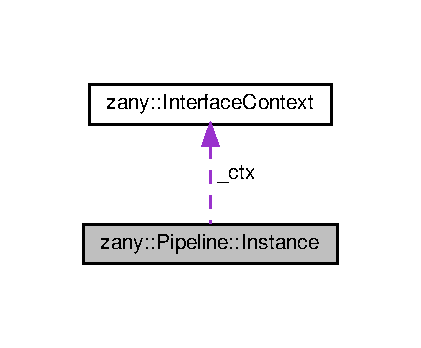
\includegraphics[width=202pt]{classzany_1_1_pipeline_1_1_instance__coll__graph}
\end{center}
\end{figure}
\subsection*{Public Attributes}
\begin{DoxyCompactItemize}
\item 
std\+::unordered\+\_\+map$<$ std\+::string, Property $>$ \hyperlink{classzany_1_1_pipeline_1_1_instance_a98f29b395ee9292ce50d9d3665ad0713}{properties}
\item 
Http\+Request \hyperlink{classzany_1_1_pipeline_1_1_instance_a1df80a693d2b107e79c7630fbc13209a}{request}
\item 
Http\+Response \hyperlink{classzany_1_1_pipeline_1_1_instance_a85b0d65a24356836b8ff33b4bec9eeca}{response}
\end{DoxyCompactItemize}


\subsection{Detailed Description}
Class instancing a \hyperlink{classzany_1_1_pipeline}{Pipeline}, launching the sets in the right order, etc... 

\subsection{Member Data Documentation}
\mbox{\Hypertarget{classzany_1_1_pipeline_1_1_instance_a98f29b395ee9292ce50d9d3665ad0713}\label{classzany_1_1_pipeline_1_1_instance_a98f29b395ee9292ce50d9d3665ad0713}} 
\index{zany\+::\+Pipeline\+::\+Instance@{zany\+::\+Pipeline\+::\+Instance}!properties@{properties}}
\index{properties@{properties}!zany\+::\+Pipeline\+::\+Instance@{zany\+::\+Pipeline\+::\+Instance}}
\subsubsection{\texorpdfstring{properties}{properties}}
{\footnotesize\ttfamily std\+::unordered\+\_\+map$<$std\+::string, Property$>$ zany\+::\+Pipeline\+::\+Instance\+::properties}

Allow data sharing between different hooks \mbox{\Hypertarget{classzany_1_1_pipeline_1_1_instance_a1df80a693d2b107e79c7630fbc13209a}\label{classzany_1_1_pipeline_1_1_instance_a1df80a693d2b107e79c7630fbc13209a}} 
\index{zany\+::\+Pipeline\+::\+Instance@{zany\+::\+Pipeline\+::\+Instance}!request@{request}}
\index{request@{request}!zany\+::\+Pipeline\+::\+Instance@{zany\+::\+Pipeline\+::\+Instance}}
\subsubsection{\texorpdfstring{request}{request}}
{\footnotesize\ttfamily Http\+Request zany\+::\+Pipeline\+::\+Instance\+::request}

Request header \mbox{\Hypertarget{classzany_1_1_pipeline_1_1_instance_a85b0d65a24356836b8ff33b4bec9eeca}\label{classzany_1_1_pipeline_1_1_instance_a85b0d65a24356836b8ff33b4bec9eeca}} 
\index{zany\+::\+Pipeline\+::\+Instance@{zany\+::\+Pipeline\+::\+Instance}!response@{response}}
\index{response@{response}!zany\+::\+Pipeline\+::\+Instance@{zany\+::\+Pipeline\+::\+Instance}}
\subsubsection{\texorpdfstring{response}{response}}
{\footnotesize\ttfamily Http\+Response zany\+::\+Pipeline\+::\+Instance\+::response}

Response header 

The documentation for this class was generated from the following file\+:\begin{DoxyCompactItemize}
\item 
lib/\+Zany/\hyperlink{_pipeline_8hpp}{Pipeline.\+hpp}\end{DoxyCompactItemize}

\hypertarget{classzany_1_1_interface_context}{}\section{zany\+:\+:Interface\+Context Class Reference}
\label{classzany_1_1_interface_context}\index{zany\+::\+Interface\+Context@{zany\+::\+Interface\+Context}}


{\ttfamily \#include $<$Context.\+hpp$>$}



Inheritance diagram for zany\+:\+:Interface\+Context\+:
\nopagebreak
\begin{figure}[H]
\begin{center}
\leavevmode
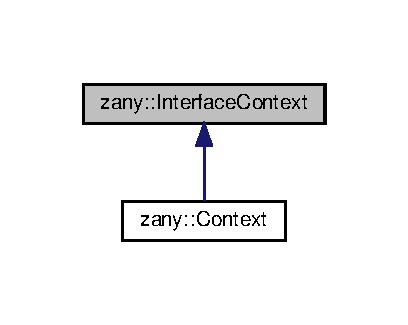
\includegraphics[width=196pt]{classzany_1_1_interface_context__inherit__graph}
\end{center}
\end{figure}
\subsection*{Public Member Functions}
\begin{DoxyCompactItemize}
\item 
virtual void \hyperlink{classzany_1_1_interface_context_a56da6cf74ba78321a0ebe0b334175176}{add\+Task} (Handler const \&handler)=0
\item 
virtual void \hyperlink{classzany_1_1_interface_context_a92f9597c6b6b7af0287a7f5178c2d063}{wait\+Until\+Empty} ()=0
\item 
virtual void \hyperlink{classzany_1_1_interface_context_a225552253490052c2fb75f05169b16a7}{run} ()=0
\item 
virtual void \hyperlink{classzany_1_1_interface_context_a13d40a4b37fca39813fe231e4081c022}{stop} ()=0
\end{DoxyCompactItemize}


\subsection{Detailed Description}
Interface Class for managing the queue of tasks 

\subsection{Member Function Documentation}
\mbox{\Hypertarget{classzany_1_1_interface_context_a56da6cf74ba78321a0ebe0b334175176}\label{classzany_1_1_interface_context_a56da6cf74ba78321a0ebe0b334175176}} 
\index{zany\+::\+Interface\+Context@{zany\+::\+Interface\+Context}!add\+Task@{add\+Task}}
\index{add\+Task@{add\+Task}!zany\+::\+Interface\+Context@{zany\+::\+Interface\+Context}}
\subsubsection{\texorpdfstring{add\+Task()}{addTask()}}
{\footnotesize\ttfamily virtual void zany\+::\+Interface\+Context\+::add\+Task (\begin{DoxyParamCaption}\item[{Handler const \&}]{handler }\end{DoxyParamCaption})\hspace{0.3cm}{\ttfamily [pure virtual]}}

Add a task


\begin{DoxyParams}{Parameters}
{\em The} & function/lambda to add to the queue \\
\hline
\end{DoxyParams}


Implemented in \hyperlink{classzany_1_1_context_a448dcb8a627491eb4c8de0f46cd13ab1}{zany\+::\+Context}.

\mbox{\Hypertarget{classzany_1_1_interface_context_a225552253490052c2fb75f05169b16a7}\label{classzany_1_1_interface_context_a225552253490052c2fb75f05169b16a7}} 
\index{zany\+::\+Interface\+Context@{zany\+::\+Interface\+Context}!run@{run}}
\index{run@{run}!zany\+::\+Interface\+Context@{zany\+::\+Interface\+Context}}
\subsubsection{\texorpdfstring{run()}{run()}}
{\footnotesize\ttfamily virtual void zany\+::\+Interface\+Context\+::run (\begin{DoxyParamCaption}{ }\end{DoxyParamCaption})\hspace{0.3cm}{\ttfamily [pure virtual]}}

Start (blocking) 

Implemented in \hyperlink{classzany_1_1_context_af7642e436736dbe466c476b56435d90f}{zany\+::\+Context}.

\mbox{\Hypertarget{classzany_1_1_interface_context_a13d40a4b37fca39813fe231e4081c022}\label{classzany_1_1_interface_context_a13d40a4b37fca39813fe231e4081c022}} 
\index{zany\+::\+Interface\+Context@{zany\+::\+Interface\+Context}!stop@{stop}}
\index{stop@{stop}!zany\+::\+Interface\+Context@{zany\+::\+Interface\+Context}}
\subsubsection{\texorpdfstring{stop()}{stop()}}
{\footnotesize\ttfamily virtual void zany\+::\+Interface\+Context\+::stop (\begin{DoxyParamCaption}{ }\end{DoxyParamCaption})\hspace{0.3cm}{\ttfamily [pure virtual]}}

Stop the context 

Implemented in \hyperlink{classzany_1_1_context_ae99b0f88172d429cc43b83effced053e}{zany\+::\+Context}.

\mbox{\Hypertarget{classzany_1_1_interface_context_a92f9597c6b6b7af0287a7f5178c2d063}\label{classzany_1_1_interface_context_a92f9597c6b6b7af0287a7f5178c2d063}} 
\index{zany\+::\+Interface\+Context@{zany\+::\+Interface\+Context}!wait\+Until\+Empty@{wait\+Until\+Empty}}
\index{wait\+Until\+Empty@{wait\+Until\+Empty}!zany\+::\+Interface\+Context@{zany\+::\+Interface\+Context}}
\subsubsection{\texorpdfstring{wait\+Until\+Empty()}{waitUntilEmpty()}}
{\footnotesize\ttfamily virtual void zany\+::\+Interface\+Context\+::wait\+Until\+Empty (\begin{DoxyParamCaption}{ }\end{DoxyParamCaption})\hspace{0.3cm}{\ttfamily [pure virtual]}}

Wait while execution queue is not empty 

Implemented in \hyperlink{classzany_1_1_context_aa611ac3befc23b58e8cef92932f21b67}{zany\+::\+Context}.



The documentation for this class was generated from the following file\+:\begin{DoxyCompactItemize}
\item 
lib/\+Zany/\hyperlink{_context_8hpp}{Context.\+hpp}\end{DoxyCompactItemize}

\hypertarget{classzany_1_1_pipeline}{}\section{zany\+:\+:Pipeline Class Reference}
\label{classzany_1_1_pipeline}\index{zany\+::\+Pipeline@{zany\+::\+Pipeline}}


{\ttfamily \#include $<$Pipeline.\+hpp$>$}

\subsection*{Classes}
\begin{DoxyCompactItemize}
\item 
class \hyperlink{classzany_1_1_pipeline_1_1_hooks}{Hooks}
\item 
class \hyperlink{classzany_1_1_pipeline_1_1_instance}{Instance}
\item 
class \hyperlink{classzany_1_1_pipeline_1_1_set}{Set}
\end{DoxyCompactItemize}
\subsection*{Public Types}
\begin{DoxyCompactItemize}
\item 
enum \hyperlink{classzany_1_1_pipeline_ab49de07eef2daaaa382e3a7b75c9e662}{Priority} \+: std\+::uint8\+\_\+t 
\item 
enum \hyperlink{classzany_1_1_pipeline_a1d41e45c2e3e9716efd9e7ae6eae99be}{Rights} \+: std\+::uint8\+\_\+t 
\end{DoxyCompactItemize}
\subsection*{Public Member Functions}
\begin{DoxyCompactItemize}
\item 
{\footnotesize template$<$typename T  = zany\+::\+Context, typename ... Args$>$ }\\void \hyperlink{classzany_1_1_pipeline_a6d37ae7b4a0045d1a9a5a8dacbd8ac29}{start\+Pipeline} (zany\+::\+Socket fd, Args \&\&...)
\item 
{\footnotesize template$<$Hooks\+::\+Decl H$>$ }\\\hyperlink{classzany_1_1_pipeline_1_1_set}{Set} \& \hyperlink{classzany_1_1_pipeline_afe387915735556acc7fc8382d9504bb7}{get\+Hook\+Set} ()
\item 
{\footnotesize template$<$Hooks\+::\+Decl H$>$ }\\void \hyperlink{classzany_1_1_pipeline_a80d8242dd8e8b94f92cc215f76427c49}{execute\+Hook} (\hyperlink{classzany_1_1_pipeline_1_1_instance}{Instance} \&instance)
\end{DoxyCompactItemize}


\subsection{Detailed Description}
Class handling the hooks to plug the modules functions to the Orchestrator Try to see it as a manager of sets of handlers, the execution is managed in the \hyperlink{classzany_1_1_pipeline_1_1_instance}{Instance} Class 

\subsection{Member Enumeration Documentation}
\mbox{\Hypertarget{classzany_1_1_pipeline_ab49de07eef2daaaa382e3a7b75c9e662}\label{classzany_1_1_pipeline_ab49de07eef2daaaa382e3a7b75c9e662}} 
\index{zany\+::\+Pipeline@{zany\+::\+Pipeline}!Priority@{Priority}}
\index{Priority@{Priority}!zany\+::\+Pipeline@{zany\+::\+Pipeline}}
\subsubsection{\texorpdfstring{Priority}{Priority}}
{\footnotesize\ttfamily enum \hyperlink{classzany_1_1_pipeline_ab49de07eef2daaaa382e3a7b75c9e662}{zany\+::\+Pipeline\+::\+Priority} \+: std\+::uint8\+\_\+t\hspace{0.3cm}{\ttfamily [strong]}}

Priority of the hook \mbox{\Hypertarget{classzany_1_1_pipeline_a1d41e45c2e3e9716efd9e7ae6eae99be}\label{classzany_1_1_pipeline_a1d41e45c2e3e9716efd9e7ae6eae99be}} 
\index{zany\+::\+Pipeline@{zany\+::\+Pipeline}!Rights@{Rights}}
\index{Rights@{Rights}!zany\+::\+Pipeline@{zany\+::\+Pipeline}}
\subsubsection{\texorpdfstring{Rights}{Rights}}
{\footnotesize\ttfamily enum \hyperlink{classzany_1_1_pipeline_a1d41e45c2e3e9716efd9e7ae6eae99be}{zany\+::\+Pipeline\+::\+Rights} \+: std\+::uint8\+\_\+t\hspace{0.3cm}{\ttfamily [strong]}}

Permissions of the hook (R\+E\+A\+D\+\_\+\+O\+N\+LY allow threading in the Pipeline()) 

\subsection{Member Function Documentation}
\mbox{\Hypertarget{classzany_1_1_pipeline_a80d8242dd8e8b94f92cc215f76427c49}\label{classzany_1_1_pipeline_a80d8242dd8e8b94f92cc215f76427c49}} 
\index{zany\+::\+Pipeline@{zany\+::\+Pipeline}!execute\+Hook@{execute\+Hook}}
\index{execute\+Hook@{execute\+Hook}!zany\+::\+Pipeline@{zany\+::\+Pipeline}}
\subsubsection{\texorpdfstring{execute\+Hook()}{executeHook()}}
{\footnotesize\ttfamily template$<$Hooks\+::\+Decl H$>$ \\
zany\+::\+Pipeline\+::execute\+Hook (\begin{DoxyParamCaption}\item[{\hyperlink{classzany_1_1_pipeline_1_1_instance}{Instance} \&}]{instance }\end{DoxyParamCaption})\hspace{0.3cm}{\ttfamily [inline]}}

Execute a hook set \mbox{\Hypertarget{classzany_1_1_pipeline_afe387915735556acc7fc8382d9504bb7}\label{classzany_1_1_pipeline_afe387915735556acc7fc8382d9504bb7}} 
\index{zany\+::\+Pipeline@{zany\+::\+Pipeline}!get\+Hook\+Set@{get\+Hook\+Set}}
\index{get\+Hook\+Set@{get\+Hook\+Set}!zany\+::\+Pipeline@{zany\+::\+Pipeline}}
\subsubsection{\texorpdfstring{get\+Hook\+Set()}{getHookSet()}}
{\footnotesize\ttfamily template$<$Pipeline\+::\+Hooks\+::\+Decl H$>$ \\
\hyperlink{classzany_1_1_pipeline_1_1_set}{Pipeline\+::\+Set} \& zany\+::\+Pipeline\+::get\+Hook\+Set (\begin{DoxyParamCaption}{ }\end{DoxyParamCaption})\hspace{0.3cm}{\ttfamily [inline]}}

Get the set of an hook \mbox{\Hypertarget{classzany_1_1_pipeline_a6d37ae7b4a0045d1a9a5a8dacbd8ac29}\label{classzany_1_1_pipeline_a6d37ae7b4a0045d1a9a5a8dacbd8ac29}} 
\index{zany\+::\+Pipeline@{zany\+::\+Pipeline}!start\+Pipeline@{start\+Pipeline}}
\index{start\+Pipeline@{start\+Pipeline}!zany\+::\+Pipeline@{zany\+::\+Pipeline}}
\subsubsection{\texorpdfstring{start\+Pipeline()}{startPipeline()}}
{\footnotesize\ttfamily template$<$typename T  = zany\+::\+Context, typename ... Args$>$ \\
zany\+::\+Pipeline\+::start\+Pipeline (\begin{DoxyParamCaption}\item[{zany\+::\+Socket}]{fd,  }\item[{Args \&\&}]{... }\end{DoxyParamCaption})\hspace{0.3cm}{\ttfamily [inline]}}

Create an instance of a \hyperlink{classzany_1_1_pipeline}{Pipeline} 

The documentation for this class was generated from the following files\+:\begin{DoxyCompactItemize}
\item 
lib/\+Zany/\hyperlink{_pipeline_8hpp}{Pipeline.\+hpp}\item 
lib/\+Zany/Pipeline.\+ipp\end{DoxyCompactItemize}

\hypertarget{classzany_1_1_pipeline_1_1_set}{}\section{zany\+:\+:Pipeline\+:\+:Set Class Reference}
\label{classzany_1_1_pipeline_1_1_set}\index{zany\+::\+Pipeline\+::\+Set@{zany\+::\+Pipeline\+::\+Set}}


{\ttfamily \#include $<$Pipeline.\+hpp$>$}

\subsection*{Public Member Functions}
\begin{DoxyCompactItemize}
\item 
{\footnotesize template$<$Priority P = Priority\+::\+L\+OW, Rights R = Rights\+::\+R\+E\+A\+D\+\_\+\+W\+R\+I\+TE$>$ }\\ID \hyperlink{classzany_1_1_pipeline_1_1_set_a1f81cf9f24022822c7c9382de470c07c}{add\+Task} (typename \+\_\+\+Function\+Type\+Selector$<$ R $>$\+::type const \&fct)
\item 
void \hyperlink{classzany_1_1_pipeline_1_1_set_ae7da91711a8148a7a1220d8dc398e1a8}{execute} (\hyperlink{classzany_1_1_pipeline_1_1_instance}{Instance} \&pipeline)
\item 
void \hyperlink{classzany_1_1_pipeline_1_1_set_a10dc8ef169ab4bf07e56d4099d2dac3c}{remove\+Task} (ID id)
\end{DoxyCompactItemize}


\subsection{Detailed Description}
A set is a group of handlers for a specific hook It sorts the handlers from their \hyperlink{classzany_1_1_pipeline_ab49de07eef2daaaa382e3a7b75c9e662}{Priority()} You don\textquotesingle{}t need to create them, \hyperlink{classzany_1_1_pipeline_afe387915735556acc7fc8382d9504bb7}{Pipeline\+::get\+Hook\+Set()} allows it 

\subsection{Member Function Documentation}
\mbox{\Hypertarget{classzany_1_1_pipeline_1_1_set_a1f81cf9f24022822c7c9382de470c07c}\label{classzany_1_1_pipeline_1_1_set_a1f81cf9f24022822c7c9382de470c07c}} 
\index{zany\+::\+Pipeline\+::\+Set@{zany\+::\+Pipeline\+::\+Set}!add\+Task@{add\+Task}}
\index{add\+Task@{add\+Task}!zany\+::\+Pipeline\+::\+Set@{zany\+::\+Pipeline\+::\+Set}}
\subsubsection{\texorpdfstring{add\+Task()}{addTask()}}
{\footnotesize\ttfamily template$<$Pipeline\+::\+Priority P, Pipeline\+::\+Rights R$>$ \\
Pipeline\+::\+Set\+::\+ID zany\+::\+Pipeline\+::\+Set\+::add\+Task (\begin{DoxyParamCaption}\item[{typename \+\_\+\+Function\+Type\+Selector$<$ R $>$\+::type const \&}]{fct }\end{DoxyParamCaption})\hspace{0.3cm}{\ttfamily [inline]}}

Add an handler to the set \mbox{\Hypertarget{classzany_1_1_pipeline_1_1_set_ae7da91711a8148a7a1220d8dc398e1a8}\label{classzany_1_1_pipeline_1_1_set_ae7da91711a8148a7a1220d8dc398e1a8}} 
\index{zany\+::\+Pipeline\+::\+Set@{zany\+::\+Pipeline\+::\+Set}!execute@{execute}}
\index{execute@{execute}!zany\+::\+Pipeline\+::\+Set@{zany\+::\+Pipeline\+::\+Set}}
\subsubsection{\texorpdfstring{execute()}{execute()}}
{\footnotesize\ttfamily void zany\+::\+Pipeline\+::\+Set\+::execute (\begin{DoxyParamCaption}\item[{\hyperlink{classzany_1_1_pipeline_1_1_instance}{Pipeline\+::\+Instance} \&}]{pipeline }\end{DoxyParamCaption})\hspace{0.3cm}{\ttfamily [inline]}}

Execute the handlers in the right order 
\begin{DoxyParams}{Parameters}
{\em pipeline} & The instance of the execution \\
\hline
\end{DoxyParams}
\mbox{\Hypertarget{classzany_1_1_pipeline_1_1_set_a10dc8ef169ab4bf07e56d4099d2dac3c}\label{classzany_1_1_pipeline_1_1_set_a10dc8ef169ab4bf07e56d4099d2dac3c}} 
\index{zany\+::\+Pipeline\+::\+Set@{zany\+::\+Pipeline\+::\+Set}!remove\+Task@{remove\+Task}}
\index{remove\+Task@{remove\+Task}!zany\+::\+Pipeline\+::\+Set@{zany\+::\+Pipeline\+::\+Set}}
\subsubsection{\texorpdfstring{remove\+Task()}{removeTask()}}
{\footnotesize\ttfamily void zany\+::\+Pipeline\+::\+Set\+::remove\+Task (\begin{DoxyParamCaption}\item[{ID}]{id }\end{DoxyParamCaption})\hspace{0.3cm}{\ttfamily [inline]}}

Remove an handler 
\begin{DoxyParams}{Parameters}
{\em id} & ID of the handler returned by \hyperlink{classzany_1_1_pipeline_1_1_set_a1f81cf9f24022822c7c9382de470c07c}{add\+Task(typename \+\_\+\+Function\+Type\+Selector$<$\+R$>$\+::type const \&fct)} \\
\hline
\end{DoxyParams}


The documentation for this class was generated from the following files\+:\begin{DoxyCompactItemize}
\item 
lib/\+Zany/\hyperlink{_pipeline_8hpp}{Pipeline.\+hpp}\item 
lib/\+Zany/Pipeline.\+ipp\end{DoxyCompactItemize}

\chapter{File Documentation}
\hypertarget{_context_8hpp}{}\section{lib/\+Zany/\+Context.hpp File Reference}
\label{_context_8hpp}\index{lib/\+Zany/\+Context.\+hpp@{lib/\+Zany/\+Context.\+hpp}}


Execution queue of the tasks.  


{\ttfamily \#include $<$queue$>$}\newline
{\ttfamily \#include $<$mutex$>$}\newline
{\ttfamily \#include $<$condition\+\_\+variable$>$}\newline
{\ttfamily \#include $<$functional$>$}\newline
{\ttfamily \#include \char`\"{}Context.\+ipp\char`\"{}}\newline
Include dependency graph for Context.\+hpp\+:\nopagebreak
\begin{figure}[H]
\begin{center}
\leavevmode
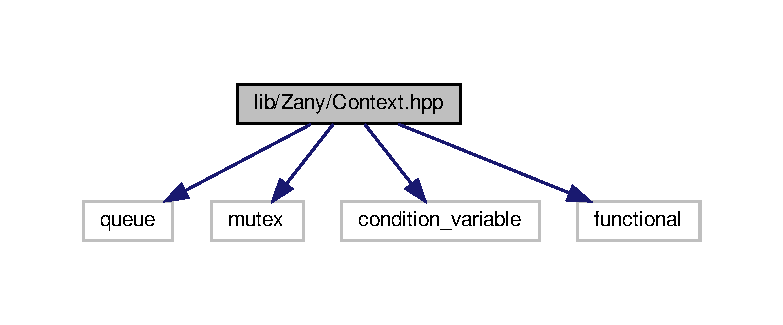
\includegraphics[width=350pt]{_context_8hpp__incl}
\end{center}
\end{figure}
This graph shows which files directly or indirectly include this file\+:\nopagebreak
\begin{figure}[H]
\begin{center}
\leavevmode
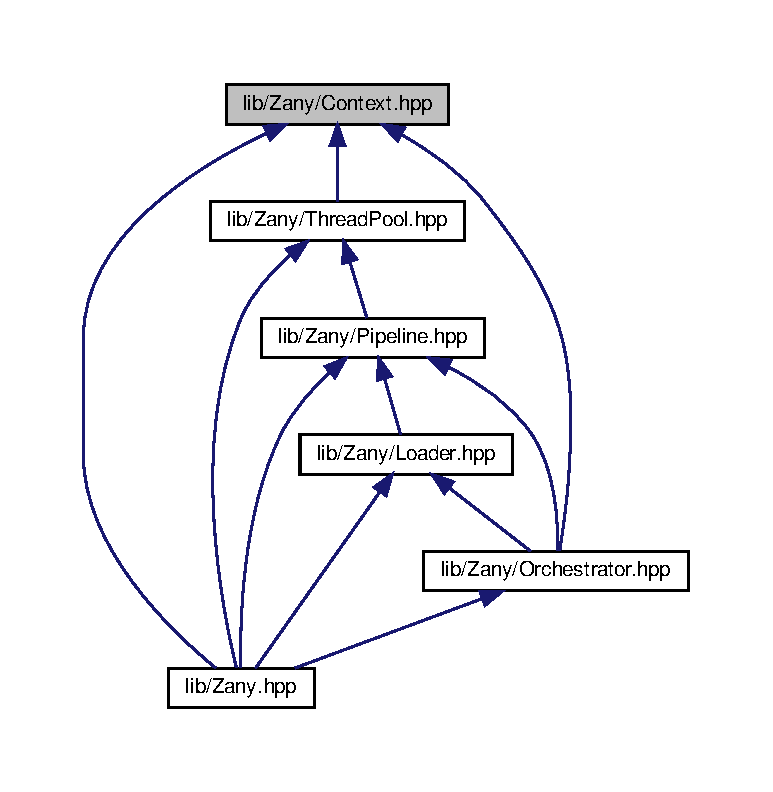
\includegraphics[width=350pt]{_context_8hpp__dep__incl}
\end{center}
\end{figure}
\subsection*{Classes}
\begin{DoxyCompactItemize}
\item 
class \hyperlink{classzany_1_1_interface_context}{zany\+::\+Interface\+Context}
\item 
class \hyperlink{classzany_1_1_context}{zany\+::\+Context}
\begin{DoxyCompactList}\small\item\em One implementation of context. \end{DoxyCompactList}\end{DoxyCompactItemize}
\subsection*{Namespaces}
\begin{DoxyCompactItemize}
\item 
 \hyperlink{namespacezany}{zany}
\end{DoxyCompactItemize}


\subsection{Detailed Description}
Execution queue of the tasks. 

\begin{DoxyAuthor}{Author}
Benjamin Viguier 
\end{DoxyAuthor}

\hypertarget{_pipeline_8hpp}{}\section{lib/\+Zany/\+Pipeline.hpp File Reference}
\label{_pipeline_8hpp}\index{lib/\+Zany/\+Pipeline.\+hpp@{lib/\+Zany/\+Pipeline.\+hpp}}


Execution queue of the tasks.  


{\ttfamily \#include $<$type\+\_\+traits$>$}\newline
{\ttfamily \#include $<$unordered\+\_\+map$>$}\newline
{\ttfamily \#include $<$exception$>$}\newline
{\ttfamily \#include $<$array$>$}\newline
{\ttfamily \#include \char`\"{}./\+Property.\+hpp\char`\"{}}\newline
{\ttfamily \#include \char`\"{}./\+Thread\+Pool.\+hpp\char`\"{}}\newline
{\ttfamily \#include \char`\"{}./\+Http\+Request.\+hpp\char`\"{}}\newline
{\ttfamily \#include \char`\"{}Pipeline.\+ipp\char`\"{}}\newline
Include dependency graph for Pipeline.\+hpp\+:\nopagebreak
\begin{figure}[H]
\begin{center}
\leavevmode
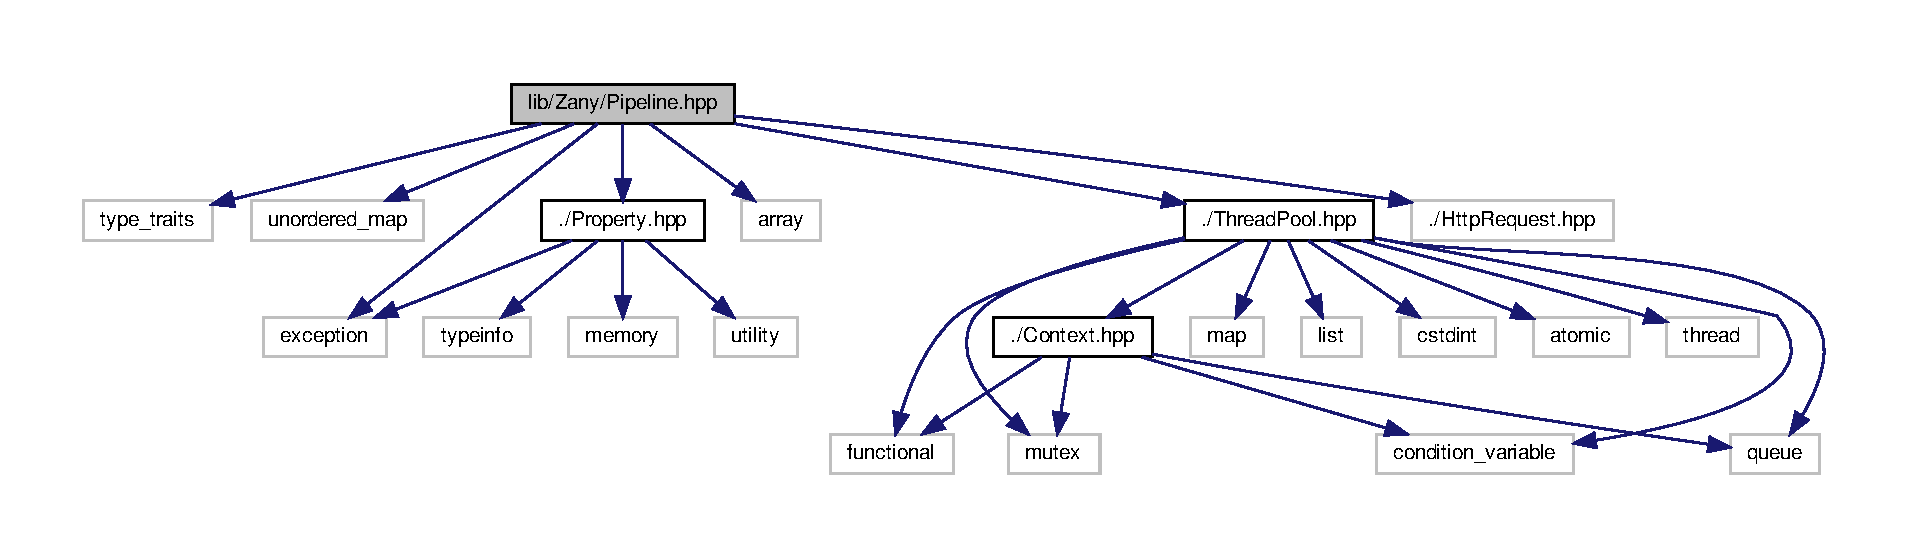
\includegraphics[width=350pt]{_pipeline_8hpp__incl}
\end{center}
\end{figure}
This graph shows which files directly or indirectly include this file\+:\nopagebreak
\begin{figure}[H]
\begin{center}
\leavevmode
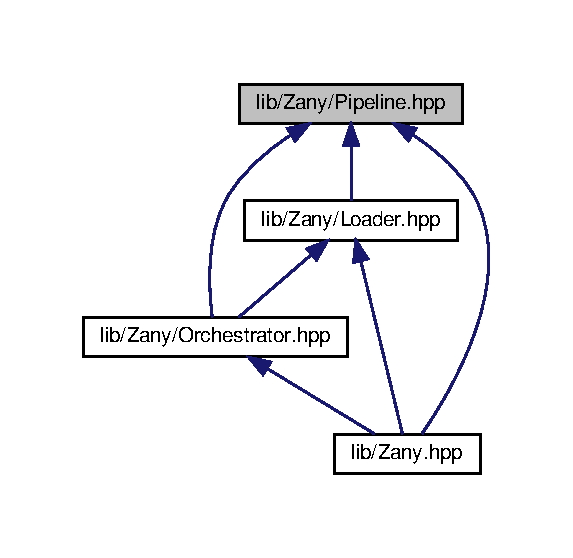
\includegraphics[width=275pt]{_pipeline_8hpp__dep__incl}
\end{center}
\end{figure}
\subsection*{Classes}
\begin{DoxyCompactItemize}
\item 
class \hyperlink{classzany_1_1_pipeline}{zany\+::\+Pipeline}
\item 
class \hyperlink{classzany_1_1_pipeline_1_1_hooks}{zany\+::\+Pipeline\+::\+Hooks}
\item 
class \hyperlink{classzany_1_1_pipeline_1_1_set}{zany\+::\+Pipeline\+::\+Set}
\item 
class \hyperlink{classzany_1_1_pipeline_1_1_instance}{zany\+::\+Pipeline\+::\+Instance}
\end{DoxyCompactItemize}
\subsection*{Namespaces}
\begin{DoxyCompactItemize}
\item 
 \hyperlink{namespacezany}{zany}
\end{DoxyCompactItemize}


\subsection{Detailed Description}
Execution queue of the tasks. 

\begin{DoxyAuthor}{Author}
Benjamin Viguier 
\end{DoxyAuthor}

%--- End generated contents ---

% Index
\backmatter
\newpage
\phantomsection
\clearemptydoublepage
\addcontentsline{toc}{chapter}{Index}
\printindex

\end{document}
